\documentclass[12pt]{amsart}
%\pagestyle{empty} 
\setlength{\topmargin}{-0.3in} % usually -0.25in
\addtolength{\textheight}{1.15in} % usually 1.25in
\addtolength{\oddsidemargin}{-0.8in}
\addtolength{\evensidemargin}{-0.8in}
\addtolength{\textwidth}{1.5in} %\setlength{\parindent}{0pt}

% macros
\usepackage{wrapfig,caption,palatino,tabularx}
\usepackage{amssymb,xspace}
\usepackage[final]{graphicx}
\usepackage[colorlinks=true]{hyperref}

\newcommand{\regfigure}[3]{\includegraphics[height=#2in,width=#3in]{#1.eps}}

\newtheorem*{lem*}{Lemma}

\newcommand{\mtt}{\texttt}
\newcommand{\mtl}[1]{{\texttt{>>#1}}}
\usepackage{alltt}
\usepackage{verbatim} % for "comment" environment
\newcommand{\mfile}[1]
{\medskip\begin{quote} \begin{alltt}\input{C:/MATLABR11/work/#1.m}\end{alltt} \end{quote}\medskip}

\newcommand{\CC}{{\mathbb{C}}}
\newcommand{\RR}{{\mathbb{R}}}
\newcommand{\eps}{\epsilon}
\newcommand{\ZZ}{{\mathbb{Z}}}
\newcommand{\ZZn}{{\mathbb{Z}}_n}
\newcommand{\NN}{{\mathbb{N}}}
\newcommand{\bu}{\mathbf{u}}
\newcommand{\bv}{\mathbf{v}}
\newcommand{\ip}[2]{\mathrm{\left<#1,#2\right>}}
\newcommand{\erf}{\operatorname{erf}}
\newcommand{\spn}{\operatorname{span}}

\newcommand{\Matlab}{\textsc{Matlab}\xspace}
\newcommand{\Octave}{\textsc{Octave}\xspace}
\newcommand{\pylab}{\textsc{pylab}\xspace}
\newcommand{\MOP}{\textsc{Matlab}\big|\textsc{Octave}\big|\textsc{pylab}\xspace}

\newcommand{\prob}[1]{\bigskip\bigskip\noindent\large\textbf{#1.} \normalsize}
\newcommand{\bookprob}[1]{\bigskip\bigskip\noindent\large\textbf{Exercise #1.} \normalsize}
\newcommand{\ppart}[1]{\medskip\noindent\large\textbf{\emph{#1})}\normalsize}

\newcommand{\textbook}{\textsc{Trefethen \& Bau}}

\begin{document}

\begin{center}
\Huge Math 661 Optimization
\end{center}

\thispagestyle{empty}
\bigskip\bigskip

\noindent \emph{instructor:} \begin{minipage}[t]{0.5\textwidth} Ed Bueler \\ \texttt{elbueler\@@alaska.edu} \end{minipage} \hfill \emph{CRN:}\, \begin{minipage}[t]{0.2\textwidth} 76523 (in-person) \\ 76522 (zoom) \end{minipage}

\medskip
\noindent \emph{course website:} \href{https://bueler.github.io/opt/}{\texttt{bueler.github.io/opt/}}

\medskip
\noindent \emph{textbook:} \begin{minipage}[t]{0.7\textwidth} Griva, Nash, \& Sofer, \emph{Linear and Nonlinear Optimization}, \\ 2nd ed, SIAM Press 2009 \end{minipage}

\bigskip
\noindent \emph{prerequisites:} calculus, linear algebra, some computer programming

\vspace{-20mm}
\hfill 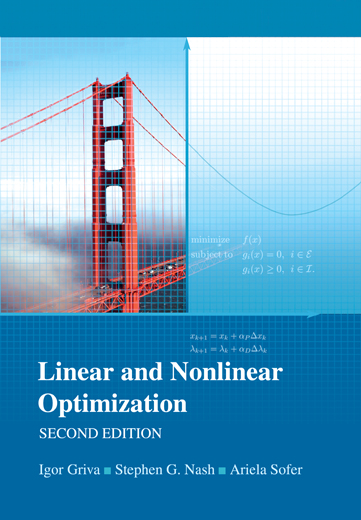
\includegraphics[height=40mm]{../images/cover.jpg}

\vspace{5mm}

\begin{wrapfigure}{l}{0.40\textwidth}
  \centering
    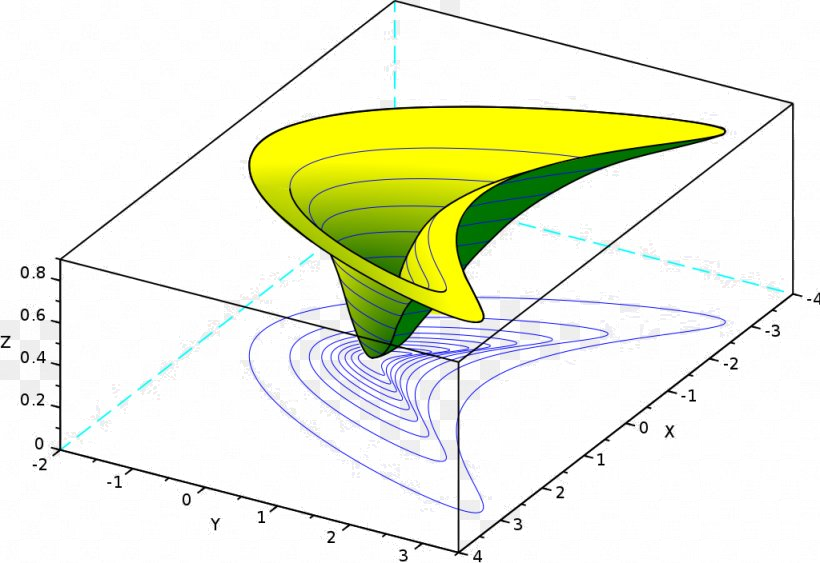
\includegraphics[width=0.38\textwidth]{../images/banana.png}
\end{wrapfigure}

Mathematical optimization is essential technology for science, engineering, and economics.  This graduate-level introduction to continuous optimization focuses on ideas, geometry, algorithms, and applications.

\smallskip
Every homework assignment includes numerical experimentation using Matlab, Python, Julia, or etc.; \emph{your choice}.  Mathematical rigor (proof) is used when appropriate, and linear algebra is always present.  There is a student-chosen project and two in-class exams.

\smallskip
At the end you will understand optimization problems as they arise in applications, know how to select algorithms, and apply optimization software based on understanding of theory and standard examples.

\smallskip
While the course is delivered hybrid, in-person attendance is preferred!

\bigskip \noindent 
\begin{minipage}[t]{0.55\textwidth} \emph{Topics:}
\begin{itemize}
\item  Linear and nonlinear optimization
\item  Iterations: Newton, quasi-Newton, CG
\item  Line search and trust region methods
\item  Linear programming
\item  Simplex and interior-point methods
\item  Equality/inequality constraints
\item KKT conditions
\end{itemize}

\bigskip
\emph{Applications:}
\begin{itemize}
\item Machine learning.
\item Inverse methods in geophysics.
\item Shape optimization in engineering.
\item Operations research.
\end{itemize}
\end{minipage}
\begin{minipage}[t]{0.45\textwidth}
\smallskip

\centering
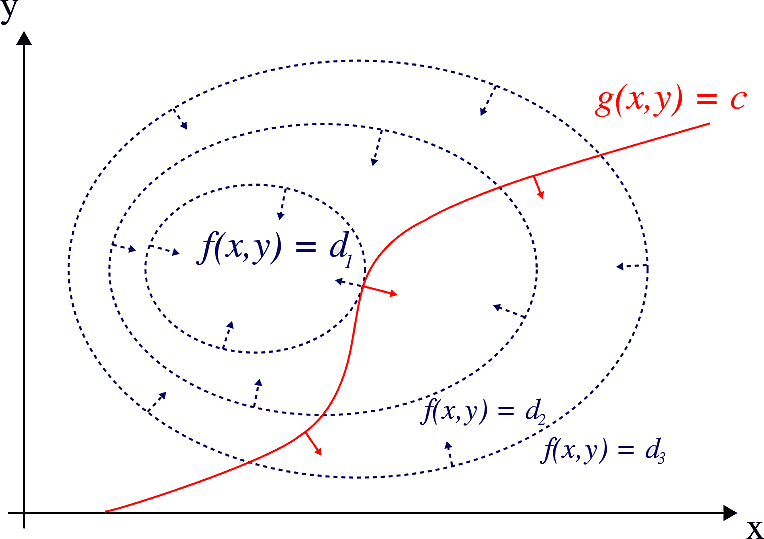
\includegraphics[height=52mm]{../images/lagrange.png}
\end{minipage}

\end{document}

